\section{Calibration}\label{sec_cnd_calib}

The calibration of the CND with beam data is done in two steps: the timing calibration, which allows us to obtain effective velocities and time offsets, which are, in turn, necessary to deduce timing and position information of the hits; and the energy calibration, in which attenuation lengths and energy conversion factors are extracted.
Table~\ref{table_cnd_constants} summarizes the calibration constants necessary to reconstruct CND hits.

\begin{table}
%\begin{center}
\begin{tabular}{|c|c|c|}
\hline
Constant name & Number of constants  & Units \\
\hline
$t_{\rm{LR}}$ & 72 & ns\\
\hline
$v_{\rm{eff}}$ & 144 & cm/ns \\
\hline
$u_{\rm{t}}$ & 72 & ns \\
\hline
$t_{\rm{LR}_{\rm{ad}}}$ & 72 & ns \\
\hline
$t_{\rm{off}}$ &72 & ns\\
\hline
$A_{\rm{L}}$ & 144 & cm\\
\hline
$MIP_{\rm{D}}$, $MIP_{\rm{I}}$ & 144 each & no units \\
\hline
\end{tabular}
%\end{center}
\caption{The constants computed in the CND calibration.}
\label{table_cnd_constants}
\end{table}

\subsection{Timing calibration}
There are four calibration constants that mist be determined as part of the CND timing calibration: the Left-Right time offset ($t_{\rm{LR}}$ and  $t_{\rm{LR}_{\rm{ad}}}$), the effective velocity ($v_{\rm{eff}}$), the propagation time in the U-turn ($u_{\rm{t}}$), and the global time offset with respect to the event start time ($t_{\rm{off}}$). The calibrations of these constants must be done in the following order: $t_{\rm{LR}}$, $v_{\rm{eff}}$, $u_{\rm{t}}$,  $t_{\rm{LR}_{\rm{ad}}}$, and finally $t_{\rm{off}}$. 
%\subsubsection{TDC to time constant}
Each of these constants is determined using charged particles from beam interactions in the target.

The raw hit times $t_{{\rm{L}}/{\rm{R}}}$ are obtained from the measured TDC channel using a slope constant of 0.0234 ns/channel for all channels.

The paddle in which the hit occurs must be determined before the calibration procedure can be applied.
The left and right times of a hit in the left paddle (we label them as $t_{{\rm{L}}/{\rm{L}}}$ and $t_{\rm{R}/{\rm{L}}}$ where the first index corresponds to the paddle under exam, while the second indicates the paddle in which the primary hit happened) are given by:
\begin{equation}
t_{{\rm{L}}/{\rm{L}}}=t_{\rm{off}}+t_{\rm{tof}}+\frac{z}{v_{\rm{eff}_L}}+t_{\rm{S}}+t_{\rm{off}_{\rm{L}}}+{\rm{TDC}}_{\rm{j}},
\end{equation}
\begin{equation}
t_{{\rm{R}/{\rm{L}}}}=t_{\rm{off}}+t_{\rm{tof}}-\frac{z}{v_{\rm{eff}_L}}+\frac{L}{v_{\rm{eff}_L}}+\frac{L}{v_{\rm{eff}_{\rm{R}}}}+u_{\rm{t}}+t_{\rm{S}}+t_{\rm{off}_{\rm{R}}}+{\rm{TDC}}_{\rm{j}},
\end{equation}
where $t_{\rm{tof}}$ is the time of flight extracted using the CVT~\cite{cvtref} path length information, $z$ is the position of the hit measured from the upstream end of the paddle, $L$ is the length of the paddle, $t_{\rm{S}}$ is the start time of the event, $t_{\rm{off}_{\rm{L}}}$ and $t_{\rm{off}_{\rm{R}}}$ are time offsets associated to the left and right coupled paddles, and ${\rm{TDC}}_{\rm{j}}$ is the TDC clock jitter.
Similarly if the hit happened in the right paddle one can write:
\begin{equation}\label{eq_time_hit_lr}
t_{{\rm{L}}/{\rm{R}}}=t_{\rm{off}}+t_{\rm{tof}}-\frac{z}{v_{\rm{eff}_{\rm{R}}}}+\frac{L}{v_{\rm{eff}_L}}+\frac{L}{v_{\rm{eff}_{\rm{R}}}}+u_{\rm{t}}+t_{\rm{S}}+t_{\rm{off}_{\rm{L}}}+{\rm{TDC}}_{\rm{j}},
\end{equation}
\begin{equation}
t_{R/R}=t_{\rm{off}}+t_{\rm{tof}}+\frac{z}{v_{\rm{eff}_{\rm{R}}}}+t_{\rm{S}}+t_{\rm{off}_{\rm{R}}}+{\rm{TDC}}_{\rm{j}}.
\end{equation}
Defining $\Delta$ and $\Delta'$ as:
\begin{equation}
\Delta=\frac{L}{v_{\rm{eff}_L}}-\frac{L}{v_{\rm{eff}_{\rm{R}}}},
\end{equation}
\begin{equation}
\Delta'=t_{\rm{L}/{\rm{X}}}-t_{\rm{R}/{\rm{X}}}+t_{\rm{off}_{\rm{R}}}-t_{\rm{off}_{\rm{L}}},
\end{equation}
where the index X can be R or L, one can compute $\Delta-\Delta'$ for both cases (hit in the left paddle or hit in the right paddle).
If the hit is in the left paddle:
\begin{equation}
\Delta'-\Delta= \frac{2z}{v_{\rm{eff}_L}} - \frac{2L}{v_{\rm{eff}_L}} -u_{\rm{t}} <0.
\end{equation}
If the hit is in the right paddle:
\begin{equation}
\Delta'-\Delta= \frac{2L}{v_{\rm{eff}_{\rm{R}}}}-\frac{2z}{v_{\rm{eff}_{\rm{R}}}} +u_{\rm{t}} >0.
\end{equation}
If $\Delta'<\Delta$, the paddle in which the hit happened is the left one, otherwise it is the right one. This procedure to determine the hit paddle depends on constants yet to be calibrated ($v_{\rm{eff}}$ and $t_{\rm{off}_{\rm{R}}}-t_{\rm{off}_{\rm{L}}}$). Therefore, at least two iterations of the calibrations of $v_{\rm{eff}}$ and $t_{\rm{off}_{\rm{R}}}-t_{\rm{off}_{\rm{L}}}$ are required.
\subsubsection{Left-right timing offset }
\paragraph{}
The Left-Right time offset refers to the time misalignement between two coupled paddles. It is detemined in two steps. The first step relies on the U-turn structure of the CND to extract an estimate of this offset $t_{\rm{LR}}$. The second step corrects this first value to obtain the real value $t_{\rm{LR}_{\rm{ad}}}$ by taking into account the effective velocities of both coupled paddles. There is one value of $t_{\rm{LR}}$ and $t_{\rm{LR}_{\rm{ad}}}$ for each pair of paddles. 

There are two different algorithms to find $t_{\rm{LR}}$ depending if the data were taken with our without magnetic field of the solenoid. 
\begin{itemize}
\item If the solenoid field is off, the U-turn light guide coupling two adjacent CND paddles induces a gap in the time difference $t_{\rm{R}}-t_{\rm{L}}$ plots. The $t_{\rm{LR}}$ constant is defined as the time difference value at the center of the gap.
\item If the solenoid is on, ``double hits'' occur. When the trajectory of a charged particle bent in the solenoid field crosses two adjacent coupled paddles, the two L/R signals have very similar TDCs (see Fig.~\ref{doublehit}). Such hits induce a peak instead of a gap in the time difference plots (see Figure \ref{LR}). $t_{\rm{LR}}$ is defined as the position of this peak.

\begin{figure}[htb]
\begin{center}
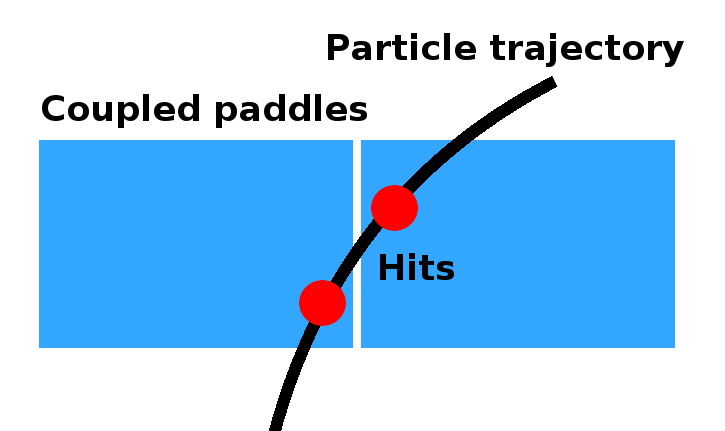
\includegraphics[width=0.45\textwidth]{Figure/doublehit.png} 
\end{center}
\caption{Double hits in the CND produced by the curved trajectory of a charged particle in the solenoid field. Both hits have similar TDCs resulting in a peak in the time difference distribution.}
\label{doublehit}
\end{figure}

\end{itemize}
Both cases are illustrated in Fig.~\ref{LR}. Typical values for the offsets are below 5 ns. $t_{\rm{LR}}$ is not used in the reconstruction, but it is nonetheless necessary to remove double hits from the subsequent calibration steps. $t_{\rm{LR}_{\rm{ad}}}$, defined below, is used in the reconstruction.
%
\begin{figure}[htb]
\begin{center}
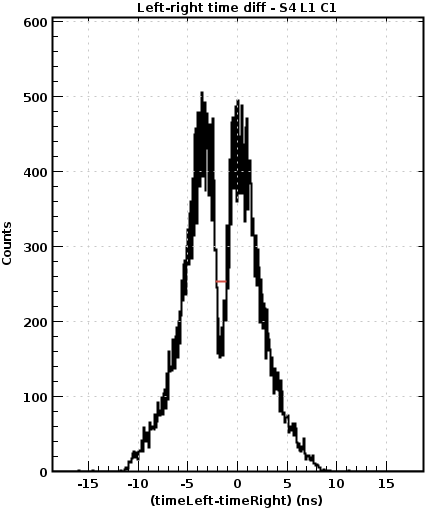
\includegraphics[width=0.3\textwidth]{Figure/nofield.png} 
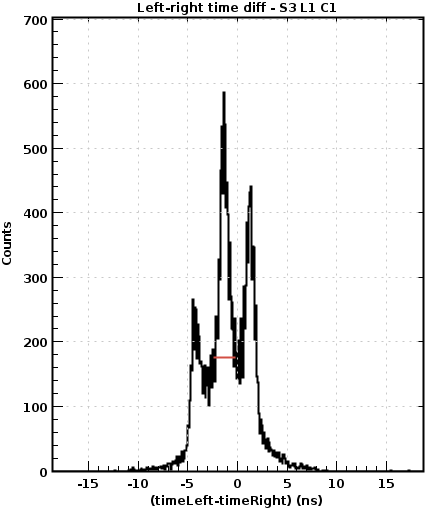
\includegraphics[width=0.3\textwidth]{Figure/field.png} 
\end{center}
\caption{Left-right time difference. The top plot is for zero solenoid field: the U-turn light guide induces a gap in the distribution. The bottom plot is for data with magnetic field: double hits, with equal TDCs, produce a peak instead of a gap.}
\label{LR}
\end{figure}
%
Once $t_{\rm{LR}}$ constants has been determined, they are corrected to account for the different effective velocities of the two coupled paddles.

For hits in the left paddle, the two associated TDCs can be expressed as:
\begin{equation}\label{time_of_hits}
t_L=t_{\rm{off}}+t_{\rm{tof}}+\frac{z}{v_{\rm{eff}_L}}+t_{\rm{S}}+t_{\rm{off}_{\rm{L}}}+{\rm{TDC}}_{\rm{j}},
\end{equation}
\begin{equation}
t_R=t_{\rm{off}}+t_{\rm{tof}}-\frac{z}{v_{\rm{eff}_L}}+\frac{L}{v_{\rm{eff}_L}}+\frac{L}{v_{\rm{eff}_{\rm{R}}}}+u_{\rm{t}}+t_{\rm{S}}+t_{\rm{off}_{\rm{R}}}+{\rm{TDC}}_{\rm{j}}.
\end{equation}

$t_{\rm{LR}_{\rm{ad}}}$ is defined as:
\begin{equation}
t_{\rm{LR}_{\rm{ad}}}=t_{\rm{off}_{\rm{R}}}-t_{\rm{off}_{\rm{L}}}.
\end{equation}

Then one can write:
\begin{equation}
\frac{t_{\rm{L}-t_{\rm{R}}}}{2}=\frac{z}{v_{\rm{eff}_{\rm{L}}}}-\frac{L}{2\cdot v_{\rm{eff}_{\rm{L}}}}-\frac{L}{2\cdot v_{\rm{eff}_{\rm{R}}}}-\frac{u_{\rm{t}}}{2}-\frac{t_{\rm{LR}_{\rm{ad}}}}{2}.
\end{equation}
The negative of the intercept of $\frac{t_{\rm{L}}-t_{\rm{R}}}{2}$ vs. $z$ is equal to:
\begin{equation}
\label{eq_1}
C_{\rm{L}}=\frac{L}{2\cdot v_{\rm{eff}_{\rm{L}}}}+\frac{L}{2\cdot v_{\rm{eff}_{\rm{R}}}}+\frac{u_{\rm{t}}}{2}+\frac{t_{\rm{LR}_{\rm{ad}}}}{2}.
\end{equation}
For hits in the right paddle, the corresponding equation reads:
\begin{equation}
\label{eq_2}
C_{\rm{R}}=\frac{L}{2\cdot v_{\rm{eff}_{\rm{R}}}}+\frac{L}{2\cdot v_{\rm{eff}_{\rm{R}}}}+\frac{u_{\rm{t}}}{2}-\frac{t_{\rm{LR}_{\rm{ad}}}}{2}.
\end{equation}
Combining equations \ref{eq_1} and \ref{eq_2}, $t_{\rm{LR}_{\rm{ad}}}$ is given by:
\begin{equation}
t_{\rm{LR}_{\rm{ad}}}=C_{\rm{L}}-C_{\rm{R}}.
\end{equation}

\subsubsection{Effective velocity }

The effective velocity $v_{\rm{eff}}$ is the speed of the light in the scintillators and the light guides. There is one $v_{\rm{eff}}$ value for each paddle. $v_{\rm{eff}}$ is obtained from the following equation:
\begin{equation}
z=(t_{\rm{L}}-t_{\rm{R}})\cdot \frac{v_{\rm{eff}}}{2} + c,
\end{equation}
where $z$ is the $z$ position of the hit in the CND with respect to the upstream end of the CND paddles and $c$ is an unknown constant. $z$ is obtained independently from the CND, using the CVT. The above equation is true for hits in left paddles. For hits in the right paddles, the sign of the time difference must be changed. $v_{\rm{eff}}$ is extracted by fitting the $\frac{t_{\rm{R}}-t_{\rm{L}}}{2}$ vs. $z$ distribution as shown in Fig.~\ref{effv}. For each slice in $z$, the position of the maximum from a Gaussian fit is plotted against $z$. The gradient of the obtained distribution gives $v_{\rm{eff}}$. The expected values for $v_{\rm{eff}}$ are around 16 cm/ns.

\begin{figure}[htb]
\begin{center}
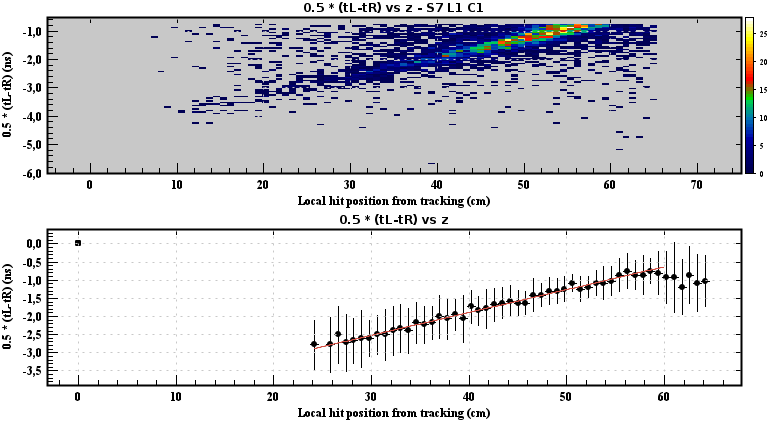
\includegraphics[width=0.48\textwidth]{Figure/veff.png} 
\end{center}
\caption{Plots used to determine the effective velocity for a CND paddle. The two plot is the raw $\frac{t_{\rm{R}}-t_{\rm{L}}}{2}$ vs $z$ and the bottom plot is the distribution showing the linear fit.}
\label{effv}
\end{figure}

\subsubsection{U-turn propagation time}

The U-turn propagation time $u_{\rm{t}}$ is the time spent by the light to travel through the U-turn light guide. It is used as a time offset on the indirect signal in the time and position reconstruction. There is one $u_{\rm{t}}$ value for each pair of paddles.
The algorithm to extract $u_{\rm{t}}$ is very similar to the one used in the $v_{\rm{eff}}$ procedure: the intercept of the $\frac{t_{\rm{R}}-t_{\rm{L}}}{2}$ vs. $z$ (see Fig.~\ref{effv}) is extracted for both coupled paddles to determine $u_{\rm{t}}$.

Recalling Eq.~\ref{time_of_hits}, the half time difference can be written :
\begin{equation}
\frac{t_{\rm{L}}-t_{\rm{R}}}{2}=\frac{z}{v_{\rm{eff}_L}}-\frac{L}{2\cdot v_{\rm{eff}_{\rm{L}}}}-\frac{L}{2\cdot v_{\rm{eff}_{\rm{R}}}}-\frac{u_{\rm{t}}}{2}-\frac{t_{\rm{LR}_{\rm{ad}}}}{2},
\end{equation}
thus the negative of the intercept of the linear fit of $\frac{t_{\rm{L}}-t_{\rm{R}}}{2}$ vs. $z$ is equal to:
\begin{equation}
\label{1}
C_{\rm{L}}=\frac{L}{2\cdot v_{\rm{eff}_{\rm{L}}}}+\frac{L}{2\cdot v_{\rm{eff}_{\rm{R}}}}+\frac{u_{\rm{t}}}{2}+\frac{t_{\rm{LR}_{\rm{ad}}}}{2}.
\end{equation}
For hits in the right paddle:
\begin{equation}
\label{2}
C_{\rm{R}}=\frac{L}{2\cdot v_{\rm{eff}_{\rm{R}}}}+\frac{L}{2\cdot v_{\rm{eff}_{\rm{R}}}}+\frac{u_{\rm{t}}}{2}-\frac{t_{\rm{LR}_{\rm{ad}}}}{2}.
\end{equation}
Combining Eqs.~\ref{1} and \ref{2}, $u_t$ is given by :
\begin{equation}
u_{\rm{t}}=C_{\rm{R}}+C_{\rm{L}}-L \left(\frac{1}{v_{\rm{eff}_{\rm{R}}}}+\frac{1}{v{_{\rm{eff}_{\rm{R}}}}}\right).
\end{equation}
The values for $u_{\rm{t}}$ are typically in the 0.5~ns - 1.5~ns range, with layer 1 values around 0.6~ns, layer 2 around 1~ns, and layer 3 around 1.4~ns.

\subsubsection{Global time offset}

The global time offset $t_{\rm{off}}$ refers to the time difference between the start time value and the vertex time computed from the CND hit time and the CVT path length information. There is one $t_{off}$ value for each pair of coupled paddles.
$t_{\rm{off}}$ is given by the following equation :
\begin{equation}
t_{\rm{off}} = \frac{t_{\rm{L}}+t_{\rm{R}}}{2} - t_{\rm{S}} - t_{\rm{tof}}
                    - \frac{L}{2} \cdot \left(\frac{1}{v_{\rm{eff}_{\rm{R}}}} + \frac{1}{v_{\rm{eff}_L}}\right) - \frac{u_{\rm{t}}}{2} - \frac{t_{\rm{LR}_{\rm{ad}}}}{2}-{\rm{TDC}}_{\rm{j}},
\end{equation}
where $t_{\rm{tof}}$ is calculated using CVT information assuming the particles are pions. For this, a negative charge is required, as most of the negative particles in the Central Detector are pions. The position of the peak of the above distribution gives $t_{\rm{off}}$. Its values depend mainly on the start time values, which is calculated using the CLAS12 FTOF system \cite{ftofref}. The variations of $t_{\rm{off}}$ between different pairs of paddles are typically below 10 ns.

%\begin{figure}[htb]
%\begin{center}
%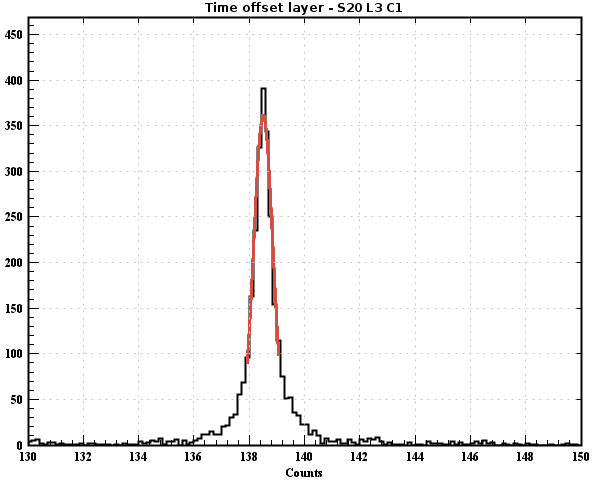
\includegraphics[width=0.45\textwidth]{Figure/timeoff.png} 
%\end{center}
%\caption{The position the peak corresponds to $t_{\rm{off}}$.}
%\label{toff}
%\end{figure}

\subsection{Energy calibration}

There are three calibration constants for the energy determination in each paddle of the CND: the attenuation length ($A_{L}$), the ADC-to-energy constants for direct minimum-ionizing particles (MIPs) ($MIP_{\rm{D}}$), and the ADC-to-energy constants for indirect MIP ($MIP_{\rm{I}}$).
These three calibration steps can be performed almost independently from the timing calibration, however, $t_{\rm{LR_{\rm{ad}}}}$ is needed to determine if an ADC signal is direct or indirect (ie the hit happened in the considered paddle or in its coupled partner).

\subsubsection{Attenuation length }

The attenuation length $A_{L}$ accounts for the light attenuation along the length of the scintillators and light guides. There is an $A_{L}$ value for each paddle.
%
For hits in the left paddle, the two associated ADCs can be written as:
\begin{equation}
\label{3}
ADC_{\rm{L}}=\frac{E}{E_0}\cdot MIP_{\rm{D}}\cdot e^{\frac{-z}{A_{L}}},
\end{equation}
\begin{equation}
\label{4}
ADC_{\rm{R}}=\frac{E}{E_0}\cdot MIP_{\rm{I}}\cdot e^{\frac{-(L-z)}{A_{\rm{L}}}},
\end{equation}
where $MIP_{\rm{D}}$ and $MIP_{\rm{I}}$ are constants defined in the Section~\ref{sec_energy_cal}, $E$ is half the energy deposited by the particle in the scintillator, and $E_0$ is half the energy deposited by a MIP in the scintillators.
$E_0$ is given by:
\begin{equation}\label{eq_def_e0}
E_0=\frac{h\cdot 1.956}{2} \rm{MeV},
\end{equation}
where $h$ is the thickness of each scintillator.
All the above equations are valid for hits in the left paddles, while for hits in the right paddles the corresponding equations are obtained by switching the indices.
From Eqs.~\ref{3} and \ref{4} the following relation is derived:
\begin{equation}
\label{5}
ln(ADC_{\rm{L}}/ADC_{\rm{R}})=c-\frac{2\cdot z}{A_{\rm{L}}},
\end{equation}
where $c$ is a constant depending on $MIP_{\rm{D}}$, $MIP_{\rm{D}}$, and $L$. $A_{\rm{L}}$ is given by the slope of the distribution in Eq.~\ref{5} as shown in Fig.~\ref{attl}. Values for $A_{\rm{L}}$ are typically around 150~cm.

\begin{figure}[htb]
\begin{center}
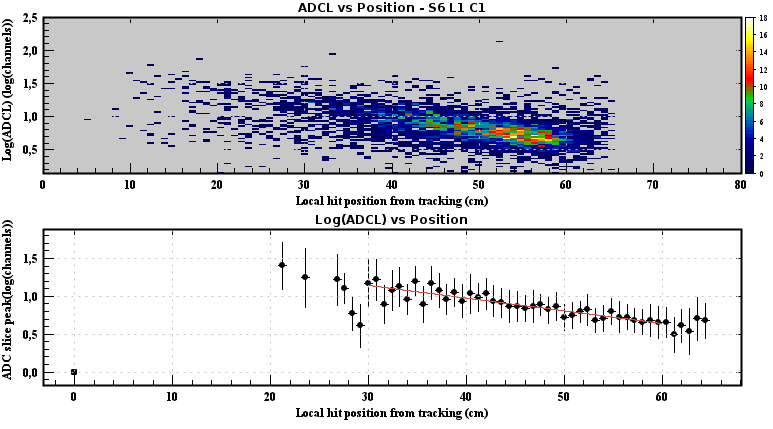
\includegraphics[width=0.48\textwidth]{Figure/attl1.png} 
\end{center}
\caption{Plots used to determine $A_{\rm{L}}$. The left plots corresponds to the left paddle and the right ones to the right paddle. The top two plots show the raw $ln(ADC_{\rm{L}}/ADC_{\rm{R}})$ vs. $z$ distributions. Slices in $z$ are fitted with a Gaussian and the mean is the plotted against $z$. The corresponding distributions and their associated linear fits are shown in the bottom two plots.}
\label{attl}
\end{figure}

\subsubsection{Energy calibration }\label{sec_energy_cal}

The final step of the calibration of the CND is the determination of the energy conversion parameters $MIP_{\rm{D}}$ and $MIP_{\rm{I}}$. There are two energy parameters for each paddle, thus there are four energy parameters for each pair of coupled paddles, denoted as $MIP_{\rm{D}}L$, $MIP_{\rm{I}}L$, $MIP_{\rm{D}}R$, $MIP_{\rm{I}}R$.

In the following, we only consider a hit in the left paddle. Equations for hits in right paddles are obtained by switching the indices. For hits in the left paddle, only $MIP_{\rm{D}}L$ and $MIP_{\rm{I}}L$ can be obtained. In the following they are referred to as $MIP_{\rm{D}}$ and $MIP_{\rm{I}}$. From Eqs.~\ref{3} and \ref{4}, one gets:
\begin{equation}
\label{6}
ln\left(\frac{ADC_{\rm{L}}}{ADC_{\rm{R}}}\right)=ln\left(\frac{MIP_{\rm{D}}}{MIP_{\rm{I}}}\right)+{\frac{L}{A_{\rm{L}}}}-\frac{2\cdot z}{A_{\rm{L}}}
\end{equation}
\begin{equation}
\label{7}
\sqrt{ADC_{\rm{L}}\cdot ADC_{\rm{R}}}=\frac{E}{E_0}\cdot \sqrt{MIP_{\rm{D}}\cdot MIP_{\rm{I}}} e^{-\frac{L}{2\cdot A_{\rm{L}}}}.
\end{equation}
From Eq.~\ref{6}, the intercept of the $ln\left(\frac{ADC_{\rm{L}}}{ADC_{\rm{R}}}\right)$ vs. $z$ distribution gives the ratio $\frac{MIP_{\rm{D}}}{MIP_{\rm{I}}}$. The same distributions as in Fig.~\ref{effv} are used to extract the intercept. The product $MIP_{\rm{D}}\cdot MIP_{\rm{I}}$ is obtained using Eq.~\ref{7} after filtering MIPs and correcting for the path travelled by the MIP in the scintillators. Indeed for MIPs, $E$ can be written as:
\begin{equation}
E=\frac{path}{h}\cdot E_0,
\end{equation}
where $path$ is the path travelled by the MIP in the scintillator, which is obtained using the CVT tracking information by extrapolating the particle trajectory at the radius of the CND hit.
Selecting MIPs and correcting for the path length removes the energy dependence from Eq.~\ref{7}, which becomes:
\begin{equation}
\sqrt{ADC_{\rm{L}}\cdot ADC_{\rm{R}}}=\frac{path}{h}\cdot \sqrt{MIP_{\rm{D}}\cdot MIP_{\rm{I}}} e^{-\frac{L}{2\cdot A_{\rm{L}}}} .
\end{equation}

The distribution of $\sqrt{ADC_{\rm{L}}\cdot ADC_{\rm{R}}}\cdot \frac{h}{path} $ is fitted with a Landau function and the position of the peak $p$ is extracted as shown in Fig.~\ref{energy}.
$MIP_{\rm{D}}$ and $MIP_{\rm{I}}$ are given by:
\begin{equation}
MIP_{\rm{D}}=\sqrt{e^{i-\frac{L}{A_{\rm{L}}}}\cdot e^{\frac{L}{A_{\rm{L}}}}\cdot p^2},
\end{equation}
\begin{equation}
MIP_{\rm{I}}=\sqrt{e^{-\left(i-\frac{L}{A_{\rm{L}}}\right)}\cdot e^{\frac{L}{A_{\rm{L}}}}\cdot p^2},
\end{equation}
where $i$ and $p$ are the intercept and peak position defined above.
$MIP_{\rm{D}}$ and $MIP_{\rm{I}}$ are typically around 2000 and 500, respectively.

In the following sections the reconstruction algorithms are described.
\begin{figure}
\begin{center}
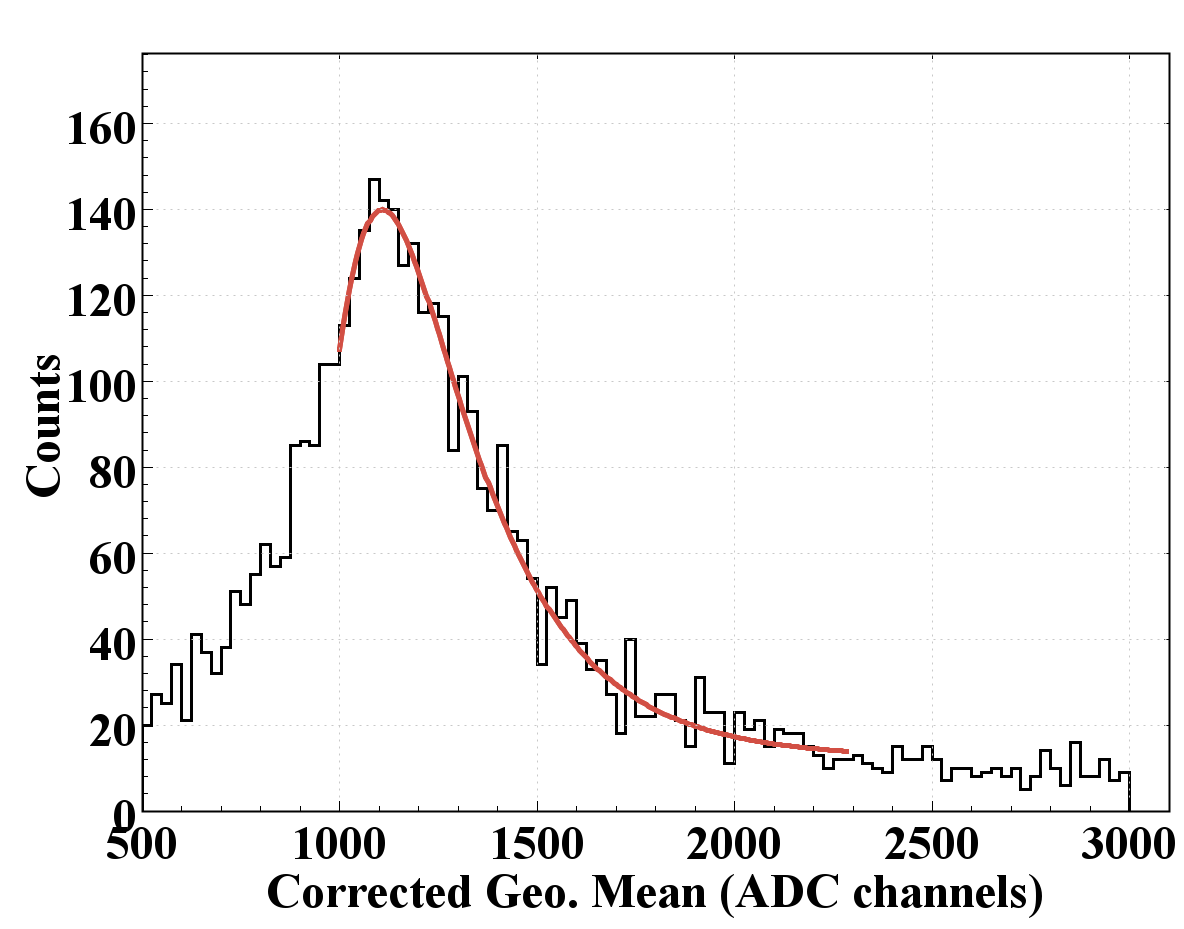
\includegraphics[width=0.45\textwidth]{Figure/energy.png} 
\caption{$\sqrt{ADC_{\rm{L}}\cdot ADC_{\rm{R}}}\cdot \frac{h}{path} $ distribution fitted with a Landau function. The events in this plot are identified as MIPs by requiring a pion. The PID is performed asking for negative charge, as most negatively charged particles in the Central Detector are pions.}
\label{energy}
\end{center}
\end{figure}
